\subsection{TENSOR PRODUCT OF AN INFINITE FAMILY OF ALGEBRAS}

Let A be a commutative ring and \((\mathrm{E}_{i})_{i\in\mathbb{I}}\) an arbitrary family of (unital) A-algebras. For every finite subset J of I, let \(E_{J}\) denote the tensor product \(\bigotimes_{i\in J}E_{i}\) of the algebras \(E_{i}\) of index \(i\in J\) ; let \(e_{i}\) denote the unit element of \(E_{i}\) and \(e_{J}=\bigotimes_{i\in J}e_{i}\) the unit element of \(E_{J}\) ; let \(f_{J,i}\) denote the canonical homomorphism \(E_{i}\to E_{J}\) for \(i\in J\) (no. 2, Proposition 5). If J, \(J'\) are two finite subsets of I such that \(J\subset J'\) , a homomorphism \(f_{J'J}:E_{J}\to E_{J'}\) is canonically derived (no. 2, Proposition 5), by the condition \(f_{J'J}\circ f_{J,i}=f_{J',i}\) for all \(i\in J\) . Moreover the uniqueness of \(f_{J'J}\) implies that if J, \(J',J''\) are three finite subsets of I such that \(J\subset J'\subset J''\) , then \(f_{J''J}=f_{J''J'}\circ f_{J'J}\) . In other words, \((\mathrm{E}_{\mathrm{J}},f_{\mathrm{J}'\mathrm{J}})\) is a direct system of A-algebras whose indexing set is the right directed set \(\mathfrak{F}(\mathbf{I})\) of finite subsets of I.

DEFINITION 5. The direct limit E of the direct system \((\mathbf{E}_{\mathbf{J}}, f_{\mathbf{J}^{\prime}\mathbf{J}})\) is called the tensor product of the family of A-algebras \((\mathbf{E}_i)_{i \in \mathbf{I}}\) .

If I is finite, E is identified with \(\bigotimes_{i\in I}E_i\) . By an abuse of notation, E is also denoted by \(\bigotimes_{i\in I}E_i\) even if I is infinite.

For every finite subset \(J\) of \(I\) , let \(f_{J}\) denote the canonical homomorphism \(\bigotimes_{i \in J} E_{i} \to \bigotimes_{i \in I} E_{i}\) (writing \(f_{i}\) instead of \(f_{(i)}\) ); if \(e\) is the unit element of \(\bigotimes_{i \in I} E_{i}\) , then \(f_{J}(e_{J}) = e\) for all \(J \in \mathfrak{F}(I)\) . It is immediate that if all the algebras \(E_{i}\) are commutative, so is \(\bigotimes_{i \in I} E_{i}\) .

PROPOSITION 8. (i) The homomorphisms \(f_{i} \colon \mathbf{E}_{i} \to \mathbf{E} = \bigotimes_{k \in \mathbf{I}} \mathbf{E}_{k}\) are such that for two indices \(i, j\) such that \(i \neq j, f_{i}(x_{i})\) and \(f_{j}(x_{j})\) commute in \(\mathbf{E}\) for all \(x_{i} \in \mathbf{E}_{i}\) and \(x_{j} \in \mathbf{E}_{j}\) ; further, \(\mathbf{E}\) is generated by the union of the subalgebras \(f_{i}(\mathbf{E}_{i})\) .

\begin{enumerate}
\def\labelenumi{(\roman{enumi})}
\setcounter{enumi}{1}
\item
  Let \(\mathbf{F}\) be an A-algebra and, for all \(i \in \mathbf{I}\) , let \(u_i: \mathbf{E}_i \to \mathbf{F}\) be an A-algebra homomorphism such that, for \(i \neq j\) , \(u_i(x_i)\) and \(u_j(x_j)\) commute in \(\mathbf{F}\) for all \(x_i \in \mathbf{E}_i\) and \(x_j \in \mathbf{E}_j\) . Then there exists one and only one A-algebra homomorphism \(u: \mathbf{E} \to \mathbf{F}\) such that \(u_i = u \circ f_i\) for all \(i \in \mathbf{I}\) .
\item
  As, for every finite subset J of I, \(f_{i} = f_{J} \circ f_{J,i}\) , the first assertion in (i) follows from no. 2, Proposition 5, taking J containing i and j; the second also follows from no. 2, Proposition 5, taking account of the fact that E is the union of the \(f_{J}(E_{J})\) when J runs through \(\mathfrak{F}(I)\) .
\item
  For every finite subset \(\mathbf{J}\) of \(\mathbf{I}\) , it follows from no. 2, Proposition 5 that there exists a unique homomorphism \(u_{\mathbf{J}}: \mathrm{E}_{\mathbf{J}} \to \mathrm{F}\) such that \(u_{\mathbf{J}} \circ f_{\mathbf{J},i} = u_{i}\) for all \(i \in J\) ; it immediately follows from this uniqueness property that, for \(J \subset J'\) , \(u_J = u_{J'} \circ f_{J'J}\) ; in other words, the \(u_J\) form a direct system of homomorphisms. Let \(u = \varinjlim u_J: E \to F\) ; then by definition \(u_J = u \circ f_J\) for every finite subset \(J\) of \(I\) and in particular \(u_i = u \circ f_i\) for all \(i \in I\) ; the uniqueness of \(u\) follows from these relations and the fact that the \(f_i(E_i)\) generate the algebra \(E\) .
\end{enumerate}

COROLLARY. Let \((\mathbf{E}_i)_{i\in \mathbf{I}}\) , \((\mathbf{E}_i')_{i\in \mathbf{I}}\) be two families of A-algebras with the same indexing set and, for all \(i\in \mathbf{I}\) , let \(u_i\colon \mathbf{E}_i\to \mathbf{E}_i'\) be an algebra homomorphism. Then there exists one and only one A-algebra homomorphism \(u\colon \bigotimes_{i\in \mathbf{I}}\mathbf{E}_i\to \bigotimes_{i\in \mathbf{I}}\mathbf{E}_i'\) such that, for all \(i\in \mathbf{I}\) , the diagram

\pandocbounded{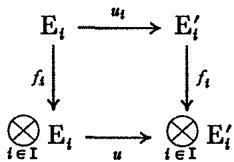
\includegraphics[keepaspectratio]{images/part003_14ac730d.jpg}}

is commutative, \(f_{i}\) and \(f_{i}^{\prime}\) denoting the canonical homomorphisms.

It suffices to apply Proposition 8 to the homomorphism \(f_{i}^{\prime} \circ u_{i}\) .

The homomorphism \(u\) defined in the Corollary to Proposition 8 is denoted by \(\bigotimes_{i \in I} u_i\) . If \(J\) is any subset of \(I\) , Proposition 8 can be applied to the family \((f_i)_{i \in J}\) of canonical homomorphisms \(f_i: E_i \to \bigotimes_{i \in I} E_i = E\) ; a canonical homomorphism \(E_J \to E\) is derived which is also denoted by \(f_J\) and which, when \(J\) is finite, coincides with the homomorphism denoted thus above.

Now let \((x_{i})_{i\in \mathbf{I}}\) be an element of \(\prod_{i\in \mathbf{I}}\mathrm{E}_i\) such that the family \((x_{i} - e_{i})_{i\in \mathbf{I}}\) has finite support H. It is immediate that, if J and \(J^{\prime}\) are two finite subsets of I containing H, then

\[
f _ {J} ((x _ {i}) _ {i \in J}) = f _ {J ^ {\prime}} ((x _ {i}) _ {i \in J ^ {\prime}}).
\]

The common value of the \(f_{\mathbf{J}}((x_i)_{i \in \mathbf{J}})\) for the finite subsets \(\mathbf{J} \supset \mathbf{H}\) of \(\mathbf{I}\) is denoted by \(\bigotimes_{i \in \mathbf{I}} x_i\) .

PROPOSITION 9. Let \((\mathbf{E}_i)_{i\in \mathbf{I}}\) be a family of A-algebras and for each \(i\in \mathbf{I}\) let \(B_{i}\) be a basis of \(\mathbf{E}_i\) such that the unit element \(e_i\) belongs to \(\overline{\mathbf{B}}_i\) . Let \(\mathbf{B}\) be the set of elements of the form \(\bigotimes_{i\in \mathbf{I}}x_i\) , where \((x_{i})\) runs through the set of elements of \(\prod_{i\in \mathbf{I}}\mathbf{B}_i\) such that the family \((x_{i} - e_{i})\) has finite support. Then \(\mathbf{B}\) is a basis of the algebra \(\bigotimes_{i\in \mathbf{I}}\mathbf{E}_i\) and this basis contains the unit element \(e\) .

For every finite subset J of I, let \(B_{J}\) be the basis of \(E_{J} = \bigotimes_{i \in J} E_{i}\) the tensor product of the bases \(B_{i}\) for \(i \in J\) (II, §3, no. 9). It follows immediately from the definitions that B is the union of the \(f_{J}(B_{J})\) when J runs through \(\mathfrak{F}(I)\) and that \(f_{J^{\prime}J}(B_{J}) \subset B_{J^{\prime}}\) when \(J \subset J^{\prime}\) ; hence \((B_{J})\) is a direct system of subsets of the \(E_{J}\) and \(B = \varinjlim B_{J}\) ; the conclusion then follows from II, §6, no. 2, Corollary to Proposition 5.

The basis B is also called the tensor product of the bases \(B_{i}\) for \(i \in I\) ; when the conditions of Proposition 9 are fulfilled, the canonical homomorphisms \(f_{J}: E_{J} \to E = \bigotimes_{i \in I} E_{i}\) are injective for every subset J of I, for if \(B_{J}\) is the basis of \(E_{J}\) the tensor product of the \(B_{i}\) for \(i \in J\) , it is immediately verified that the restriction of \(f_{J}\) to \(B_{J}\) is injective and maps \(B_{J}\) onto a subset of B.

